\documentclass{beamer}
\mode<presentation>
{
  \usetheme{default}
  \usecolortheme{default}
  \usefonttheme{default}
  \setbeamertemplate{navigation symbols}{}
  \setbeamertemplate{caption}[numbered]
} 

\usepackage{polski}
\usepackage[utf8]{inputenc}
\usepackage[T1]{fontenc}

\resetcounteronoverlays{saveenumi}


\title[M2.2]{Zarządzanie Systemami Informatycznymi}
\author{Mikołaj Buczak, Karolina Woźniak}
\institute{Politechnika Śląska}
\date{\today}

\begin{document}

\begin{frame}
  \titlepage
\end{frame}


\begin{frame}{System informatyczny}
     System informatyczny to zbiór powiązanych ze sobą elementów, w którym ma miejsce przepływ lub przetwarzanie danych w sposób zautomatyzowany, najczęściej przy użyciu techniki komputerowej.
\end{frame}

\begin{frame}{System informatyczny}
     Przykładem systemu informatycznego wspomagającym pracę kawiarenki internetowej jest "Activity Monitor"
\end{frame} 

\begin{frame}{Activity Monitor}
     Activity Monitor to oprogramowanie wykorzystywane w firmach, bibliotekach, szkołach, więc doskonale sprawdzi się również w kawiarence internetowej  do monitorowania poczynań użytkowników komputerów. Daje możliwość:
     \begin{itemize}
         \item podglądu obrazów pulpitów
         \item rejestrowania informacji o odwiedzanych stronach internetowych i uruchamianych aplikacjach.
     \end{itemize}
    
\end{frame}

\begin{frame}{System wspomagający zdalną edukację}
    \begin{itemize}
        \item Komunikator
        \item szybki dostęp do ocen
        \item podział na przedmioty
        \item możliwość wysyłania prac
        \item możliwość przeprowadzenie testu
    \end{itemize}
\end{frame}

\begin{frame}{PZE}
    Komunikator pozwala na szybką komunikację zarówno między studentami jak i prowadzącymi zajęcia. Dzięki nie mu nie jest konieczne używanie e-maili, które nie każdy na bieżąco sprawdza. Pozwala również na komentarze ze strony wykładowców do treści przesyłanych przez studentów.
\end{frame}
\begin{frame}{Dostęp do ocen}
    Studenci na bieżąco mają dostęp do swoich ocen końcowych i cząstkowych.
\end{frame}

\begin{frame}{Podział na przedmioty}
    Każdy prowadzący ma możliwość utworzenia kursu dla danego przedmiotu. Student aby móc korzystać z materiałów zawartych w kursach musi się na nie zapisać. Wykładowcy na bieżąco mogą dodawać tam materiały dydaktyczne.
\end{frame}
\begin{frame}{Wysyłanie prac}
    Studenci poprzez Platformę Zdalnej Edukacji w ramach danego kursu mogą wysyłać wszystkie zadanie, kolokwia, egzaminy. 
    Wystarczy przeciągnąć plik do wysłania w odpowiednie miejsce
    \begin{figure}[H!]
        \centering
        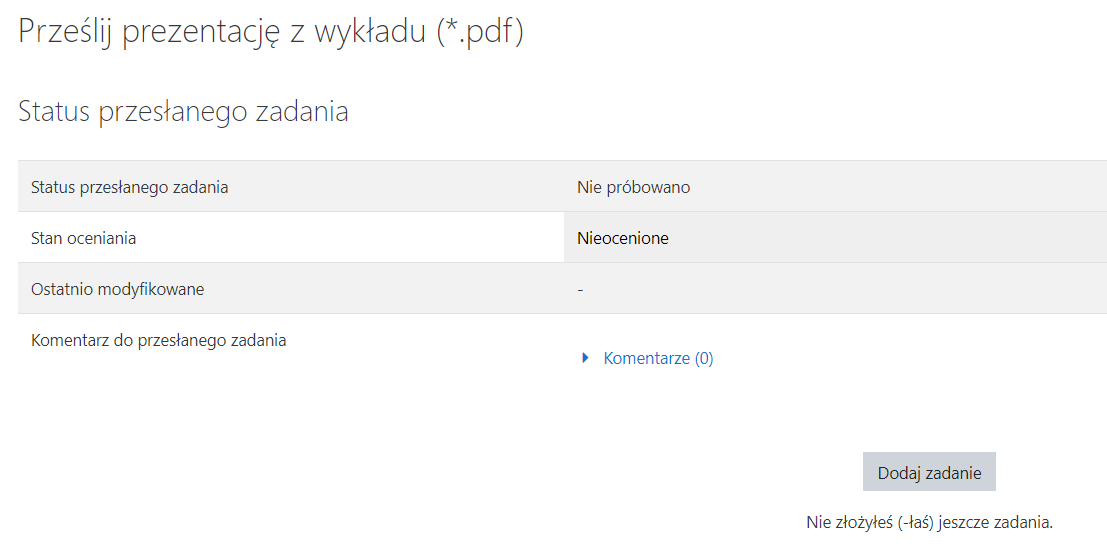
\includegraphics[width=\textwidth]{przesylanie.PNG}
    
        
    \end{figure}
\end{frame}

\begin{frame}{Testy on-line}
    Platforma umożliwia przeprowadzanie testów on-line i automatyczne sprawdzanie odpowiedzi, student od razu po zakończeniu sprawdzianu dostaje wynik.
\end{frame}

\begin{frame}{Specyfikacja techniczna systemem Canva}
    \begin{enumerate}
        \item[1] Każda wizytówka oparta jest o dane i osiągnięcia indywidualnego studenta.
        \item[2] Aplikacja jest prosta i intuicyjna w użytkowaniu, nowoczesna i przejrzysta; charakteryzuje
    się zminimalizowanym czasem załadowania.
        \item[3] Działa prawidłowo w następujących systemach: MS Windows, GNU/Linux, MacOS.
        \item[4] Aplikacja zostanie zoptymalizowana do rozdzielczości poziomej 720 pikseli
    z wyłączonym skalowaniem w przypadku gdy użytkownik używa większej rozdzielczości.
    \end{enumerate}
\end{frame}

\begin{frame}{Specyfikacja techniczna systemem Canva}
    \begin{enumerate}
        \item[5] aplikacja jest responsywna - dostosowuje się do rozdzielczości urządzenia na jakim jest
    oglądana (telefon komórkowy, tablet, PC).
        \item[6] Kodowanie polskich znaków w aplikacji internetowym odbywa się wg standardu UTF-8.
        \item[7] Strona po wdrożeniu posiada kod zgodny z SOLID.
    \end{enumerate}
\end{frame}
\begin{frame}{Specyfikacja techniczna systemem Canva}
    \begin{enumerate}
        \item[8] Strona internetowa wyposażona jest w mechanizm automatycznej archiwizacji dokumentów
    z określonym czasem publikacji i możliwości korzystania z archiwum. Administrator ma możliwość
    swobodnej decyzji dotyczącej przedłużenia czasu publikacji, automatycznej archiwizacji lub
    usunięcia wizytówek.
        \item[9] W trakcie prezentacji dowolnej wizytówki w aplikacji, użytkownik ma możliwość zmiany wielkości
    tekstu (pomniejszenie/powiększenie czcionki); wydruku; ściągnięcia pliku do pobrania; wysyłki
    treści e-mailem w formie funkcji „Wyślij znajomym" - wysyłanie do znajomego bezpośrednio ze stron
    WWW, rekomendacji z informacją o istnieniu danej podstrony.
        \item[10] Aplikacja zawiera wyszukiwarkę umożliwiającą użytkownikowi przeszukiwanie
    zarówno proste, jak i zaawansowane - z uwzględnieniem kryteriów.
    \end{enumerate}
\end{frame}

\begin{frame}{Specyfikacja techniczna systemem Canva}
    \begin{enumerate}
        \item[11] Aplikacja umożliwia upload zdjęć oraz elementów multimedialnych (audio, video,
    flash).
        \item[12] Strona posiada mechanizm umożliwiający wyświetlenie informacji o czasowej niedostępności
    serwisu z powodów technicznych.
        \item[13] Mapa aplikacji tworzona jest automatycznie.
    \end{enumerate}
\end{frame}

\end{document}